\section{Amdahl's Law}

\begin{frame}[t]{Amdahl's Law}
\begin{itemize}
  \item Performance increase obtained using a faster execution mode
        is limited by the fraction of time that the mode can be used.

  \mode<presentation>{\pause\vfill}
  \item \textgood{Speedup}:
    \begin{itemize}
      \item Ratio between improved performance ($P(I)$) and original performance ($P(O)$).
    \end{itemize}
\end{itemize}

\begin{displaymath}
S = \frac{P(I)}{P(O)}
\end{displaymath}

\begin{displaymath}
S = \frac{T(O)}{T(I)}
\end{displaymath}
\end{frame}

\begin{frame}[t]{Execution time}
\begin{columns}[T]
\begin{column}{0.35\textwidth}
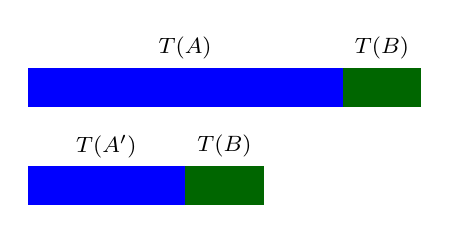
\begin{tikzpicture}
\tikzset{
    etiqueta/.style={text centered, font=\footnotesize} 
}  
\fill(0,1.25) [fill=blue] rectangle (4,1.75);
\fill(4,1.25) [fill=green!40!black] rectangle (5,1.75);
\node[etiqueta] at (2,2) {$T(A)$};
\node[etiqueta] at (4.5,2) {$T(B)$};
\fill(0,0) [fill=blue] rectangle (2,0.5);
\fill(2,0) [fill=green!40!black] rectangle (3,0.5);
\node[etiqueta] at (1,0.75) {$T(A')$};
\node[etiqueta] at (2.5,0.75) {$T(B)$};
\end{tikzpicture}
\end{column}
\pause
\begin{column}{.65\textwidth}
\begin{small}
\begin{displaymath}
F=\frac{T(A)}{T} =\pause
\quad \Rightarrow \quad 1 - F = \frac{T(B)}{T} \pause
\quad \Rightarrow \quad T(B) = (1 - F) T 
\end{displaymath}
\pause
\begin{displaymath}
S(i)=\frac{T(A)}{T(A')} \pause
\quad \Rightarrow \quad T(A') = \frac{T(A)}{S(i)}
\end{displaymath}
\end{small}
\end{column}
\end{columns}

\pause
\begin{small}
\begin{displaymath}
T'=T(A')+T(B)= \pause
\frac{T(A)}{S(i)}+(1-F) \times T
\end{displaymath}
\pause
\begin{displaymath}
T'=\frac{F \times T}{S(i)} + (1-F) \times T
\end{displaymath}
\pause
\begin{displaymath}
T'=T \times \Big[ (1 - F) + \frac{F}{S(i)} \Big]
\end{displaymath}
\end{small}
\end{frame}

\begin{frame}[t]{Amdahl's Law}
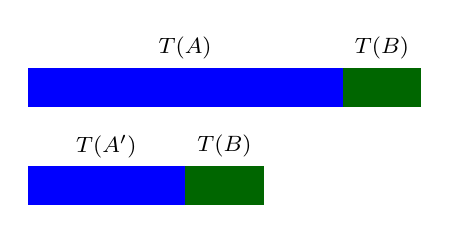
\begin{tikzpicture}
\tikzset{
    etiqueta/.style={text centered, font=\footnotesize} 
}  
\fill(0,1.25) [fill=blue] rectangle (4,1.75);
\fill(4,1.25) [fill=green!40!black] rectangle (5,1.75);
\node[etiqueta] at (2,2) {$T(A)$};
\node[etiqueta] at (4.5,2) {$T(B)$};
\fill(0,0) [fill=blue] rectangle (2,0.5);
\fill(2,0) [fill=green!40!black] rectangle (3,0.5);
\node[etiqueta] at (1,0.75) {$T(A')$};
\node[etiqueta] at (2.5,0.75) {$T(B)$};
\end{tikzpicture}
\begin{small}
\begin{displaymath}
T'=T \times \Big[ (1 - F) + \frac{F}{S(i)} \Big]
\end{displaymath}
\pause
\begin{displaymath}
S=\frac{T}{T'}=\pause
\frac{T}{T \times \Big[ (1 - F) + \frac{F}{S(i)} \Big]} =\pause
\frac{1}{(1 - F) + \frac{F}{S(i)}}
\end{displaymath}
\end{small}
\begin{itemize}
  \item \textmark{\emph{Speedup}} depends \textbf{exclusively} on
        the \textgood{improvement fraction} and the \textgood{speedup of the improvement}.
\end{itemize}
\end{frame}

\begin{frame}[t]{Case 1}
\begin{itemize}
  \item A Web server distributes its time between: 
    \begin{itemize}
      \item \textmark{Computing}: 40%.
      \item \textmark{I/O}: 60%.
    \end{itemize}
  \item When replaced by another machine that can perform
        computing 10 times faster, which is the global \emph{speedup}?
\end{itemize}
\mode<presentation>{\pause\vfill}
\begin{block}{Solution}
\begin{displaymath}
S=
\frac{1}{0.6+\frac{0.4}{10}} =
\frac{1}{0.64} =
1.5625
\end{displaymath}
\end{block}
\end{frame}

\begin{frame}[t]{Case 2}
\begin{itemize}
  \item An application has a parallelizable part that takes
        50\% of the execution time.
    \begin{itemize}
      \item Assuming that this part can be fully parallelized
            with 32 processors, which is the maximum speedup?
    \end{itemize}
\end{itemize}
\mode<presentation>{\pause\vfill}
\begin{block}{Solution}
\begin{displaymath}
S=
\frac{1}{0.5 + \frac{0.5}{32}} =
\frac{1}{0.515625} =
1.9393
\end{displaymath}
\end{block}
\end{frame}

\begin{frame}[t]{Speedup evolution}
\begin{tikzpicture}
\begin{axis}[xlabel=processors,ylabel=speedup, 
minor y tick num=1,
legend style = {
at={(1.02, 1)},
anchor=north west
},
width=0.85\textwidth, height=0.85\textheight,
xmin=0,xmax=128,
ymin=0,ymax=10]
\addplot [domain=1:128,color=red,very thick] {1 / (0.5 + (0.5 / x))};
\addlegendentry{F=0.5}
\addplot [domain=1:128,color=orange,very thick] {1 / (0.4 + (0.6 / x))};
\addlegendentry{F=0.6}
\addplot [domain=1:128,color=green, very thick] {1 / (0.3 + (0.7 / x))};
\addlegendentry{F=0.7}
\addplot [domain=1:128,color=yellow, very thick] {1 / (0.2 + (0.8 / x))};
\addlegendentry{F=0.8}
\addplot [domain=1:128, color=blue, very thick] {1 / (0.1 + (0.9 / x))};
\addlegendentry{F=0.9}
\end{axis}
\end{tikzpicture}
\end{frame}

\begin{frame}[t]{Amdahl's Law consequences}
\begin{itemize}
  \item The greater the fraction of improvement (F),
        the more effective the improvement is.

  \mode<presentation>{\pause\vfill}
  \item To improve a complex system you must optimize the
        elements that are used most of the time (most common case).

  \mode<presentation>{\pause\vfill}
  \item Optimization application:
    \begin{itemize}
      \item \textmark{Within the processor}: 
            in the data path.
      \item \textmark{In the instruction set}: 
            the execution of most frequent instructions.
      \item \textmark{In the design of memory hierarchy, programming and compilation}:
            exploiting reference locality.
        \begin{itemize}
          \item 10\% of code is executed for 90\% of time.
        \end{itemize}
    \end{itemize}
\end{itemize}
\end{frame}
